%%%%%%%% ICML 2025 — MutGAT Submission %%%%%%%%%%%%%%%%%%%%%%%%%%%%%%%%%%%%%%%%

\documentclass{article}

\usepackage{microtype}
\usepackage{graphicx}
\usepackage{subfigure}
\usepackage{booktabs}
\usepackage{hyperref}
\usepackage{multirow}

\newcommand{\theHalgorithm}{\arabic{algorithm}}

\usepackage[accepted]{icml2025}

\usepackage{amsmath}
\usepackage{amssymb}
\usepackage{mathtools}
\usepackage{amsthm}
\usepackage[capitalize,noabbrev]{cleveref}

%%%%%%%%%%%%%%%%%%%%%%%%%%%%%%%%
% THEOREMS
%%%%%%%%%%%%%%%%%%%%%%%%%%%%%%%%
\theoremstyle{plain}
\newtheorem{theorem}{Theorem}[section]
\newtheorem{proposition}[theorem]{Proposition}
\newtheorem{lemma}[theorem]{Lemma}
\newtheorem{corollary}[theorem]{Corollary}
\theoremstyle{definition}
\newtheorem{definition}[theorem]{Definition}
\newtheorem{assumption}[theorem]{Assumption}
\theoremstyle{remark}
\newtheorem{remark}[theorem]{Remark}

\icmltitlerunning{MutGAT: Pathway-Enriched HGAT for MTB Resistance Prediction}

\begin{document}

\twocolumn[
\icmltitle{MutGAT: Knowledge-Graph-Enriched Heterogeneous Graph Attention\\
           for Antibiotic Resistance Prediction in \textit{Mycobacterium tuberculosis}}

\icmlsetsymbol{equal}{*}

\begin{icmlauthorlist}
\icmlauthor{Akshat Shah}{equal,yyy}
\icmlauthor{Manidhar Sukasi}{equal,yyy}
\end{icmlauthorlist}

\icmlaffiliation{yyy}{IIIT Hyderabad}

\icmlcorrespondingauthor{Akshat Shah}{akshat.shah@research.iiit.ac.in}

\icmlkeywords{graph attention networks, tuberculosis, antibiotic resistance,
              genomics, KEGG pathways, heterogeneous graphs,
              drug susceptibility testing, ablation study}

\vskip 0.3in
]

\printAffiliationsAndNotice{\icmlEqualContribution}

%%%%%%%%%%%%%%%%%%%%%%%%%%%%%%%%%%%%%%%%%%%%%%%%%%%%%%%%%%%%%%%%%%%%%%%%%%%
%  ABSTRACT
%%%%%%%%%%%%%%%%%%%%%%%%%%%%%%%%%%%%%%%%%%%%%%%%%%%%%%%%%%%%%%%%%%%%%%%%%%%

\begin{abstract}
Predicting antibiotic resistance in \textit{Mycobacterium tuberculosis} (MTB) from whole-genome sequencing data is critical for guiding effective therapy. Heterogeneous graph attention networks (HGATs) have shown promise by modelling isolate--SNP relationships, but existing approaches are limited to first-line drugs and operate on a flat bipartite graph that ignores the biological pathway context linking resistance genes. We present \textbf{MutGAT}, which enriches the HGAT framework with structured knowledge from the KEGG pathway database, adding pathway, KEGG Orthology (KO), and drug node types with biologically grounded edges to form a multi-level heterogeneous graph, and extends prediction to both first- and second-line drugs. Through a systematic four-model ablation study on the CRyPTIC dataset (12{,}279 isolates, 8 anti-TB drugs), we isolate the contribution of each layer of biological knowledge. The full MutGAT model achieves the best mean sensitivity across drugs (82.6\% vs.\ 80.8\% for the SNP-only baseline) and the highest AUROC on 6 of 8 drugs, with the largest gains on second-line drugs where baseline performance is lowest. Attention score analysis across the heterogeneous graph provides multi-level interpretability, identifying resistance-associated genes and quantifying pathway contributions for each drug.
\end{abstract}

%%%%%%%%%%%%%%%%%%%%%%%%%%%%%%%%%%%%%%%%%%%%%%%%%%%%%%%%%%%%%%%%%%%%%%%%%%%
%  1. INTRODUCTION
%%%%%%%%%%%%%%%%%%%%%%%%%%%%%%%%%%%%%%%%%%%%%%%%%%%%%%%%%%%%%%%%%%%%%%%%%%%

\section{Introduction}
\label{sec:intro}

Tuberculosis (TB) reclaimed its position as the leading cause of death from a single infectious agent globally in 2023, claiming an estimated 1.25~million lives \citep{who2024tb}. Drug-resistant TB remains a major threat. Of an estimated 400{,}000 people who developed multidrug-resistant or rifampicin-resistant TB (MDR/RR-TB) in 2023, only 44\% were diagnosed and treated \citep{who2024tb}. MDR-TB is defined as resistance to at least the two first-line drugs isoniazid (INH) and rifampicin (RIF). The emergence of drug-resistant MTB, driven by treatment lapses and compensatory bacterial evolution, creates an urgent need for faster and more accurate resistance prediction.

Conventional phenotypic drug susceptibility testing (DST) requires weeks of culture-based incubation, creating diagnostic delays that impede timely treatment \citep{who2024tb}. Whole-genome sequencing (WGS) delivers results within days directly from sputum samples, and the WHO endorsed targeted next-generation sequencing for genotypic DST as an alternative to phenotypic methods in 2024 \citep{who2024ngs}. Widely used genotypic tools such as TB-Profiler \citep{phelan2019tbprofiler} and Mykrobe \citep{hunt2019mykrobe} rely on curated catalogues of known resistance-conferring mutations, most notably the WHO 2021 catalogue \citep{walker2022who}. While highly specific, these approaches cannot detect resistance arising from novel mutations outside catalogued loci, and they model each mutation independently, ignoring the epistatic and co-occurrence interactions that characterise MTB resistance biology.

Machine learning has emerged as a promising paradigm to move beyond fixed mutation catalogues. Early classifiers trained on SNP presence--absence vectors demonstrated meaningful improvements over direct-association methods \citep{yang2018ml}, while platforms such as GenTB \citep{groschel2021gentb} extended this to larger cohorts using Random Forest and Wide-and-Deep Neural Network models. More recently, whole-genome XGBoost and neural network models have pushed further by operating on genome-wide variants and discovering novel resistance-associated mutations through explainability methods \citep{pal2025mlmtb}. TB-DROP \citep{wang2024tbdrop} demonstrated that end-to-end deep learning frameworks consuming whole-genome mutation matrices could achieve competitive performance with fast per-sample runtimes.

\citet{yang2021hgat} introduced HGAT--AMR, the first heterogeneous graph attention network for MTB resistance prediction. By representing isolates and SNPs as nodes in a bipartite graph (with SNP nodes typed by their host gene) and applying a dual-attention mechanism at the type and node levels, HGAT--AMR achieved state-of-the-art AUROC on INH and RIF while providing interpretable gene- and SNP-level attention scores. However, HGAT--AMR operates on a flat isolate--SNP graph with no explicit encoding of the biological pathways that link resistance genes. Genes involved in the same metabolic pathway, such as \textit{embA}, \textit{embB}, and \textit{embC} in the arabinosyltransferase pathway targeted by ethambutol, have no direct connection in the graph. Information between them flows only indirectly through shared isolate nodes, which limits the model's ability to leverage pathway-level biological priors.

We introduce \textbf{MutGAT}, which enriches the heterogeneous graph with structured biological knowledge from the KEGG database \citep{kanehisa2000kegg}. Our key contributions are:
\begin{enumerate}
    \item A \textbf{KEGG-enriched heterogeneous graph} that extends the isolate--SNP bipartite structure with pathway, KEGG Orthology (KO), and drug node types connected through biologically grounded edges, enabling direct message passing between functionally related gene representations.
    \item A \textbf{four-model ablation study} that systematically isolates the contribution of each layer of biological knowledge: \textsc{HGAT-Base} (SNP-only baseline), \textsc{HGAT-Path} (pathway-enriched), \textsc{HGAT-KO} (KO-bridged), and the full \textsc{MutGAT} (drug-aware).
    \item A \textbf{multi-level interpretability analysis} providing gene-level and pathway-level attention scores that identify resistance-associated genes and quantify pathway contributions per drug, extending prior work to the pathway scale.
\end{enumerate}

%%%%%%%%%%%%%%%%%%%%%%%%%%%%%%%%%%%%%%%%%%%%%%%%%%%%%%%%%%%%%%%%%%%%%%%%%%%
%  2. RELATED WORK
%%%%%%%%%%%%%%%%%%%%%%%%%%%%%%%%%%%%%%%%%%%%%%%%%%%%%%%%%%%%%%%%%%%%%%%%%%%

\section{Related Work}
\label{sec:related}

\subsection{Catalogue-Based Genotypic DST}
The molecular foundations of MTB drug resistance were established in the 1990s with the identification of spontaneous chromosomal mutations in specific target genes. Seminal discoveries mapped \textit{katG} to isoniazid resistance \citep{zhang1992katg}, \textit{rpoB} to rifampicin resistance \citep{telenti1993rpob}, \textit{inhA} as the target for both isoniazid and ethionamide \citep{banerjee1994inha}, and \textit{pncA} to pyrazinamide resistance \citep{scorpio1996pnca}. These insights drove the development of Direct Association tools like TB-Profiler and Mykrobe. Recently, these efforts culminated in the comprehensive WHO catalogue of MTB complex mutations, which provides a globally standardised library of resistance-associated variants across 13 anti-TB drugs \citep{walker2022who}.

\subsection{Machine Learning and Deep Learning Approaches}
To overcome the limitations of rule-based methods, a range of machine learning and deep learning models have been applied to WGS data. Classical approaches include Support Vector Machines with 3D structural protein annotations for identifying pan-genomic resistance signatures \citep{kavvas2018machine}, Logistic Regression and Gradient Tree Boosting with dimensionality reduction for difficult drugs such as pyrazinamide \citep{kouchaki2019application}, and gradient-boosted trees that explicitly model co-occurrent resistance markers \citep{deelder2019machine}. As datasets have expanded, deep learning architectures have been adopted to capture non-linear epistatic interactions: Wide-and-Deep Neural Networks jointly memorise canonical resistance loci while generalising from rare variants \citep{chen2019beyond}, and platforms such as GenTB \citep{groschel2021gentb} and TB-DROP \citep{wang2024tbdrop} have translated these advances into clinical utility. The CRyPTIC consortium has further pushed the field by predicting continuous minimum inhibitory concentrations \citep{cryptic2022mic}. Despite these advances, both families treat mutations as flat feature vectors, leaving the relational structure between variants, genes, and pathways unexploited.

\subsection{Graph Neural Networks}
Graph neural networks (GNNs) generalise deep learning to graph-structured data by iteratively aggregating information from local neighbourhoods \citep{kipf2017gcn}. Graph Attention Networks (GATs) extend this with learnable, neighbour-specific attention weights, improving performance and providing edge-level interpretability \citep{velickovic2018gat}. Heterogeneous graph attention networks (HGATs) further generalise GATs to graphs with multiple node and edge types via type-aware projections and hierarchical attention \citep{wang2019han}, making them a natural fit for jointly modelling heterogeneous biological entities such as samples, variants, genes, and pathways.

Within MTB resistance prediction, \citet{yang2021hgat} proposed HGAT--AMR, which applies this framework to a bipartite isolate--SNP graph with per-gene-typed SNP nodes and dual-level attention to produce interpretable multi-drug isolate embeddings.

\subsection{KEGG Pathways}
The KEGG database \citep{kanehisa2000kegg} provides manually curated pathway maps that organise genes into functional modules, together with KEGG Orthology (KO) groups that link genes across organisms by shared function. While KEGG pathways are widely used for downstream enrichment analysis of resistance-associated genes, they have not previously been incorporated as an explicit relational signal in MTB resistance prediction. Existing approaches treat resistance genes as independent features or flat node sets, ignoring the pathway-level organisation that links genes such as \textit{embA}/\textit{embB}/\textit{embC} (arabinosyltransferase) or \textit{gyrA}/\textit{gyrB} (DNA gyrase). Our work fills this gap by directly embedding KEGG pathways and KO groups as nodes in a heterogeneous graph.

%%%%%%%%%%%%%%%%%%%%%%%%%%%%%%%%%%%%%%%%%%%%%%%%%%%%%%%%%%%%%%%%%%%%%%%%%%%
%  3. METHOD
%%%%%%%%%%%%%%%%%%%%%%%%%%%%%%%%%%%%%%%%%%%%%%%%%%%%%%%%%%%%%%%%%%%%%%%%%%%

\section{MutGAT}
\label{sec:method}

In this section we describe MutGAT, a heterogeneous graph attention network that enriches a bipartite isolate--SNP graph with structured biological knowledge from the KEGG database. We begin by motivating the graph representation of MTB genomic data, then describe how the graph is constructed in progressive stages, from a baseline SNP graph through to the full pathway-enriched model. The attention mechanism, pathway context readout, and training procedure are described thereafter. This progressive construction defines our four-model ablation: each successive model adds one layer of biological knowledge, allowing us to isolate the contribution of pathways, orthology groups, and drug-level structure.

\subsection{Representing Genomic Data as a Graph}
\label{sec:graph_motivation}

Each MTB isolate carries a variable number of single nucleotide polymorphisms (SNPs) distributed across a panel of 23 resistance-associated genes. Conventional ML methods flatten this structure into a fixed-length binary vector, with one element per possible SNP, discarding the grouping of SNPs by gene and the relationships between genes. Graph neural networks offer a natural alternative. By representing each isolate and each SNP as a node in a graph, and connecting them with edges that encode which SNPs are present in which isolate, we preserve the variable-length, hierarchically organised nature of the data.

We construct a \emph{heterogeneous} graph in which different genes correspond to different node types. An isolate node and a \textit{katG} SNP node are connected by a different edge type than an isolate node and an \textit{rpoB} SNP node. This heterogeneity is key: it allows the attention mechanism to learn gene-specific importance weights, effectively discovering which genes matter most for predicting resistance to each drug.

\subsection{Graph Construction}
\label{sec:graph}

\begin{figure*}[!t]
\vskip 0.05in
\begin{center}
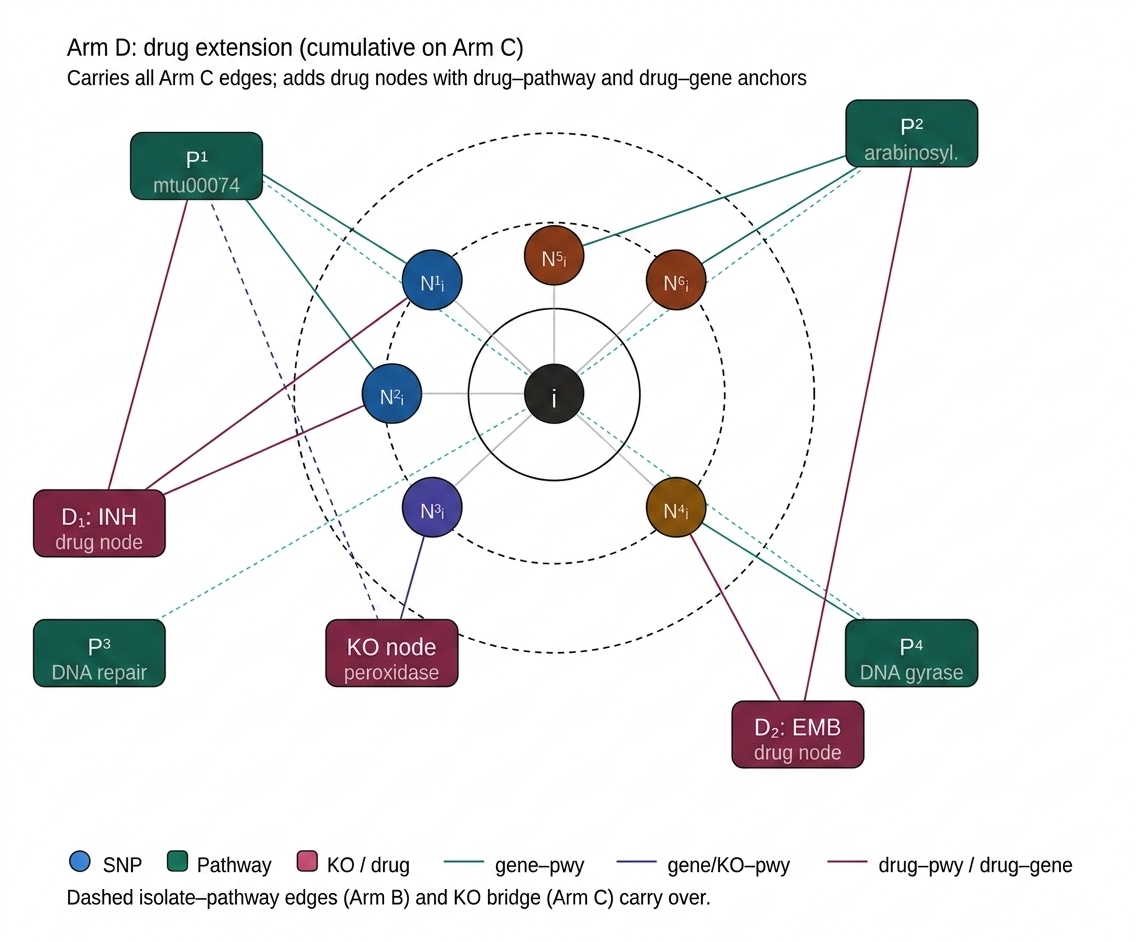
\includegraphics[width=\textwidth]{fig_mutgat_graph.jpg}
\end{center}
\vskip -0.15in
\caption{Illustrative MutGAT heterogeneous graph for a single isolate (centre). SNP nodes sit in gene-specific type spaces; pathway, KO, and drug nodes anchor biological relationships. Line styles distinguish edge types as in the legend; earlier ablation stages omit subsets of nodes and edges (\cref{tab:arms}).}
\label{fig:mutgat-graph}
\vskip -0.05in
\end{figure*}

We build the graph in four progressive stages, each of which defines one model in our ablation study. \cref{tab:arms} summarises the node types, edge types, and classification head used by each model; \cref{fig:mutgat-graph} sketches the cumulative heterogeneous topology for the full \textsc{MutGAT} graph (drug extension on top of pathway and KO structure).

\paragraph{Stage 1: The SNP graph (\textsc{HGAT-Base}).}
The foundation is a bipartite graph connecting isolate nodes to SNP nodes. Let $\mathcal{V}_I = \{s_1, \ldots, s_N\}$ denote the $N = 12{,}279$ isolate nodes. For each of the 23 resistance-associated genes $g$, a separate set of SNP nodes $\mathcal{V}_g = \{v^g_1, \ldots, v^g_{n_g}\}$ represents the unique SNPs observed in that gene across the dataset. A bidirectional edge is placed between isolate $s_i$ and SNP node $v^g_j$ whenever that SNP is present in isolate $s_i$. SNP nodes belonging to different genes reside in distinct type spaces and share no direct edges. The only path between a \textit{katG} SNP and an \textit{rpoB} SNP passes through their shared isolate neighbours. This model serves as our baseline.

\paragraph{Stage 2: Adding pathway nodes (\textsc{HGAT-Path}).}
A limitation of \textsc{HGAT-Base} is that genes in the same metabolic pathway, such as \textit{embA}, \textit{embB}, and \textit{embC} (which encode successive enzymes in the arabinosyltransferase pathway targeted by ethambutol), can only exchange information through shared isolate nodes. This is a two-hop indirect path. To address this, we introduce $P = 22$ pathway nodes drawn from the KEGG database for \textit{M.~tuberculosis} (organism code \texttt{mtu}). We exclude the two largest hub pathways (\texttt{mtu01100} ``Metabolic pathways'' and \texttt{mtu01110} ``Biosynthesis of secondary metabolites'') because they connect to nearly all genes non-specifically, diluting the pathway signal and causing over-smoothing. We explicitly include the mycolic acid biosynthesis pathway (\texttt{mtu00074}), which is mechanistically central to INH resistance through the KatG--InhA--FabG1 axis.

Two new edge types connect these pathway nodes to the rest of the graph. First, \textbf{isolate--pathway edges}: an isolate $s_i$ is connected to pathway $p$ if it carries any SNP in a gene that belongs to $p$. These edges allow the model to contextualise an isolate's mutational profile within the pathway landscape. Second, \textbf{gene--pathway edges}: every SNP node of gene $g$ is connected directly to each pathway that $g$ participates in. These are the most consequential edges in the enrichment, creating a direct one-hop path between genes in the same pathway (for example, \textit{gyrA} SNP $\to$ DNA gyrase pathway $\to$ \textit{gyrB} SNP), which enables the attention mechanism to propagate resistance-relevant information along biologically meaningful routes.

To prevent information cycling through the pathway hub in deeper layers, since isolate $\to$ pathway $\to$ isolate shortcuts could otherwise bypass the gene-level structure, we mask the pathway$\to$isolate edge direction in the second HGAT layer.

\paragraph{Stage 3: Bridging with KO nodes (\textsc{HGAT-KO}).}
Not all resistance genes map directly to KEGG pathways. To bring these ``pathway-orphan'' genes into the pathway neighbourhood, we add $K = 19$ KEGG Orthology (KO) nodes. Each KO group represents a set of genes with shared evolutionary origin and conserved function. SNP nodes of a gene connect to the KO node for that gene's orthologous group, and KO nodes in turn connect to the pathways they participate in. This creates a two-hop bridge (orphan gene SNP $\to$ KO $\to$ pathway), integrating genes that would otherwise remain isolated from the pathway structure.

\paragraph{Stage 4: Drug-aware classification (\textsc{MutGAT}).}
The full model adds $D = 8$ drug nodes, one per predicted antibiotic. Each drug node is connected to its known target pathways and target gene SNP nodes, as annotated in the KEGG knowledge graph. At classification time, each drug uses a per-drug pathway mask that restricts the pathway attention to only those pathways associated with that drug in KEGG. Each drug also has its own classifier head. This drug-aware design forces the pathway context to focus on biologically relevant pathways rather than distributing attention uniformly.

\begin{table}[t]
\caption{Summary of the four ablation models. Each successive model cumulatively adds node types and edges to the graph.}
\label{tab:arms}
\vskip 0.1in
\begin{center}
\begin{small}
\begin{tabular}{llll}
\toprule
Model & Nodes added & Edges added & Classifier \\
\midrule
\textsc{HGAT-Base} {\small(baseline)} & iso, SNP$_g${\small($\times$23)} & iso$\leftrightarrow$SNP & shared MLP \\
\textsc{HGAT-Path} & + pathway{\small(22)} & + iso$\leftrightarrow$pwy & + pathway \\
              &                       & + gene$\leftrightarrow$pwy & \ \ context \\
\textsc{HGAT-KO}   & + KO{\small(19)}      & + gene$\leftrightarrow$KO & + pathway \\
              &                       & + KO$\leftrightarrow$pwy & \ \ context \\
\textsc{MutGAT} & + drug{\small(8)}   & + drug$\leftrightarrow$pwy & per-drug \\
              &                       & + drug$\leftrightarrow$gene & \ \ heads \\
\bottomrule
\end{tabular}
\end{small}
\end{center}
\vskip -0.1in
\end{table}

\subsection{Node Feature Initialisation}
\label{sec:features}

Before training, each node must be assigned an initial feature vector. The quality of these initialisations matters because they determine the starting point from which the attention mechanism learns.

\paragraph{SNP embeddings.}
We draw an analogy between SNP co-occurrence patterns and word co-occurrence in natural language: just as words that appear in similar contexts tend to have related meanings, SNPs that co-occur across isolates may share functional relevance. We compute a pointwise mutual information (PMI) matrix over the SNP co-occurrence statistics, retain only positive values (PPMI), and factorise the result via truncated singular value decomposition (SVD) to produce a 64-dimensional embedding for each SNP. To avoid information leakage during cross-validation, these co-occurrence statistics are computed exclusively from training-fold isolates, so each fold operates with its own set of SNP embeddings.

\paragraph{Isolate embeddings.}
Each isolate's feature vector is obtained by element-wise max-pooling over the PMI+SVD embeddings of all SNPs present in that isolate. The max-pool aggregator preserves the most distinctive SNP signal present in the isolate.

\paragraph{Pathway and KO features.}
Rather than using uninformative identity vectors, we initialise pathway nodes with gene-membership binary vectors: a pathway's feature has dimension equal to the number of gene types in the graph, with a 1 in position $j$ if gene $g_j$ belongs to that pathway. This directly encodes the biological composition of each pathway. KO nodes are similarly initialised with pathway-membership vectors indicating which pathways each orthologous group participates in.

\paragraph{Drug features.}
Drug nodes are initialised with one-hot identity vectors of dimension $D = 8$.

\subsection{Heterogeneous Graph Attention}
\label{sec:hgat}

The core of MutGAT is a stack of two heterogeneous graph attention layers. The attention mechanism operates identically in all four ablation models; what differs is only the set of node and edge types present in the graph. This ensures that any performance differences are attributable to the graph structure rather than to architectural changes.

For a given edge type $r = (\tau_s, \text{rel}, \tau_d)$ connecting source type $\tau_s$ to destination type $\tau_d$, each edge type has its own learnable projection matrix $\mathbf{W}_r \in \mathbb{R}^{d' \times d}$ and attention vector $\mathbf{a}_r \in \mathbb{R}^{2d'}$. For a destination node $v$ and its neighbour $u$ under edge type $r$, the attention coefficient is:
\begin{equation}
    \alpha_{uv}^{(r)} = \frac{
        \exp\!\bigl(\text{LeakyReLU}\!\bigl(\mathbf{a}_r^\top [\mathbf{W}_r \mathbf{h}_u \,\|\, \mathbf{W}_r \mathbf{h}_v]\bigr)\bigr)
    }{
        \sum_{u' \in \mathcal{N}_r(v)} \exp\!\bigl(\text{LeakyReLU}\!\bigl(\mathbf{a}_r^\top [\mathbf{W}_r \mathbf{h}_{u'} \,\|\, \mathbf{W}_r \mathbf{h}_v]\bigr)\bigr)
    },
\label{eq:att}
\end{equation}
where $\|$ denotes concatenation and $\mathcal{N}_r(v)$ is the set of $v$'s neighbours under edge type $r$. The attention scores are normalised per edge type via softmax, so the model learns separate importance distributions for each relationship (e.g., isolate--\textit{katG} vs. isolate--\textit{rpoB}).

Messages from all edge types incident on $v$ are then summed and passed through layer normalisation and an ELU activation:
\begin{equation}
    \mathbf{h}_v' = \text{ELU}\!\left(\text{LayerNorm}\!\left(\sum_{r \in \mathcal{R}_v} \sum_{u \in \mathcal{N}_r(v)} \alpha_{uv}^{(r)}\, \mathbf{W}_r\, \mathbf{h}_u \right)\right),
\label{eq:update}
\end{equation}
where $\mathcal{R}_v$ is the set of edge types with $v$ as a destination. We use $K=2$ attention heads (concatenated), hidden dimension $d=128$, and dropout $p=0.3$ after each layer.

The second layer uses the same mechanism but, in \textsc{HGAT-Path}, \textsc{HGAT-KO}, and \textsc{MutGAT}, excludes the pathway$\to$isolate edge direction. This selective masking prevents the pathway nodes from acting as hubs that wash out the gene-level attention structure. It preserves the benefits of pathway connectivity while avoiding over-smoothing.

\subsection{Pathway Context Readout}
\label{sec:classifier}

After the two HGAT layers, we obtain isolate representations from both layers and concatenate them as $\mathbf{z}_i = [\mathbf{h}_i^{(1)} \| \mathbf{h}_i^{(2)}]$. This skip connection ensures the classifier sees both the fine-grained first-layer features and the more abstract second-layer representations, mitigating information loss from deeper propagation.

In \textsc{HGAT-Base}, the concatenated vector $\mathbf{z}_i$ is passed directly to a shared two-layer MLP classifier ($128 \to 128 \to D_{\text{drugs}}$) with ReLU activation and dropout.

In \textsc{HGAT-Path} and \textsc{HGAT-KO}, a pathway context vector is appended to $\mathbf{z}_i$ before classification. This vector is computed via scaled dot-product attention between the second-layer isolate embedding and all pathway node embeddings:
\begin{equation}
    \mathbf{c}_i = \sum_{p=1}^{P} \frac{\exp(\mathbf{h}_i^{(2)} \cdot \mathbf{h}_p^{(2)} / \sqrt{d})}{\sum_{p'} \exp(\mathbf{h}_i^{(2)} \cdot \mathbf{h}_{p'}^{(2)} / \sqrt{d})} \; \mathbf{h}_p^{(2)},
\label{eq:pwy_ctx}
\end{equation}
followed by a two-layer MLP to produce a refined context $\tilde{\mathbf{c}}_i$. The classifier input becomes $[\mathbf{h}_i^{(1)} \| \mathbf{h}_i^{(2)} \| \tilde{\mathbf{c}}_i]$. Intuitively, this attention readout asks: ``given this isolate's learned representation, which pathways are most relevant for predicting its resistance profile?'' The resulting attention weights provide a pathway-level interpretation of each prediction.

In \textsc{MutGAT}, the pathway context is computed separately for each drug. For drug $d$, a drug-specific learned attention head scores each pathway, but the softmax is masked to include only pathways annotated as associated with drug $d$ in KEGG. Pathways outside this mask receive zero attention weight. Each drug then has its own classifier head operating on $[\mathbf{h}_i^{(1)} \| \mathbf{h}_i^{(2)} \| \tilde{\mathbf{c}}_i^{(d)}]$, producing a single logit per drug. This design encodes the prior that different drugs act through different pathways, focusing each drug's prediction on the pathways most likely to be mechanistically relevant.

\subsection{Training}
\label{sec:training}

The model is trained with binary cross-entropy loss, masked to ignore missing labels (drugs not tested for a given isolate):
\begin{equation}
\begin{split}
    \mathcal{L} = -\frac{1}{|\mathcal{M}|} \sum_{(i,d) \in \mathcal{M}}
        \bigl[\, &w_d^+ \, y_{id} \log \sigma(l_{id}) \\
        &+ (1 - y_{id}) \log(1 - \sigma(l_{id})) \,\bigr],
\end{split}
\label{eq:loss}
\end{equation}
where $\mathcal{M}$ is the set of valid (isolate, drug) pairs with available phenotypes, $w_d^+$ is the per-drug positive class weight (ratio of susceptible to resistant samples, clamped to $[1, 10]$), and $\sigma$ denotes the sigmoid function. This masked loss allows the model to learn from isolates with incomplete drug-resistance profiles without discarding partially-labelled data.

Optimisation uses Adam with learning rate $5 \times 10^{-4}$, weight decay $10^{-4}$, and gradient clipping at norm~1.0. Training runs for up to 180 epochs with early stopping on mean validation AUROC (patience 20). Per-drug classification thresholds are tuned on the validation set by grid search over $[0.1, 0.9]$ to maximise F1-score.

%%%%%%%%%%%%%%%%%%%%%%%%%%%%%%%%%%%%%%%%%%%%%%%%%%%%%%%%%%%%%%%%%%%%%%%%%%%
%  4. EXPERIMENTS
%%%%%%%%%%%%%%%%%%%%%%%%%%%%%%%%%%%%%%%%%%%%%%%%%%%%%%%%%%%%%%%%%%%%%%%%%%%

\section{Experiments}
\label{sec:experiments}

\subsection{Dataset}

We evaluate on the CRyPTIC dataset \citep{cryptic2022mic}, comprising 12{,}279 \textit{M.~tuberculosis} isolates with WGS data and binarised phenotypes (resistant/susceptible) for 8 anti-TB drugs. \cref{tab:prevalence} shows the class distribution. Variant calling extracts SNPs from 23 established resistance-associated genes with quality filters (QUAL $\geq$ 20, allele frequency $\geq$ 0.75).

\begin{table}[t]
\caption{Drug resistance prevalence in the CRyPTIC evaluation cohort (per-fold test set averages). First-line drugs above the rule.}
\label{tab:prevalence}
\vskip 0.1in
\begin{center}
\begin{small}
\begin{tabular}{lccc}
\toprule
Drug & $n_R$ & $n_S$ & \%R \\
\midrule
INH & 1{,}181 & 1{,}231 & 49.0 \\
RIF & 937 & 1{,}481 & 38.7 \\
EMB & 452 & 1{,}666 & 21.4 \\
ETH & 345 & 1{,}885 & 15.5 \\
\midrule
LEV & 429 & 2{,}002 & 17.6 \\
MXF & 345 & 2{,}092 & 14.1 \\
KAN & 224 & 2{,}200 & 9.2 \\
AMI & 176 & 2{,}236 & 7.3 \\
\bottomrule
\end{tabular}
\end{small}
\end{center}
\vskip -0.1in
\end{table}

\subsection{Evaluation Protocol}

All four models share identical evaluation to ensure fair comparison.
\textbf{Cross-validation} uses 5-fold outer CV with multi-label stratified splits, balancing all 8 drug phenotypes simultaneously. An inner 4-fold split produces train (60\%), validation (20\%), and test (20\%) partitions.
\textbf{Per-fold embeddings}: PMI+SVD embeddings are recomputed for each fold using only training-fold isolates.
\textbf{Early stopping} is applied on mean validation AUROC with patience 20.
\textbf{Threshold tuning}: per-drug classification thresholds are optimised on the validation set only.

\subsection{Metrics}

We report per-drug AUROC, sensitivity (recall for the resistant class), specificity, and F1-score, averaged over 5 folds with standard deviations.

%%%%%%%%%%%%%%%%%%%%%%%%%%%%%%%%%%%%%%%%%%%%%%%%%%%%%%%%%%%%%%%%%%%%%%%%%%%
%  5. RESULTS
%%%%%%%%%%%%%%%%%%%%%%%%%%%%%%%%%%%%%%%%%%%%%%%%%%%%%%%%%%%%%%%%%%%%%%%%%%%

\section{Results}
\label{sec:results}

\subsection{AUROC Comparison}

\cref{tab:auroc} reports AUROC across all four models and eight drugs. All models achieve strong discrimination (AUROC $>$ 0.90 on every drug). \textsc{MutGAT} achieves the highest AUROC on 6 of 8 drugs, with a mean AUROC of 94.08\% compared to 93.91\% for \textsc{HGAT-Base}. The improvements are concentrated on second-line drugs: LEV (+0.54\,pp), MXF (+0.53\,pp), and ETH (+0.09\,pp).

\begin{table*}[t]
\caption{AUROC (\%) across ablation models. Mean $\pm$ std over 5-fold CV. Best per drug in \textbf{bold}. First-line drugs above the rule.}
\label{tab:auroc}
\vskip 0.1in
\begin{center}
\begin{small}
\begin{tabular}{lcccc}
\toprule
Drug & \textsc{HGAT-Base} & \textsc{HGAT-Path} & \textsc{HGAT-KO} & \textsc{MutGAT} \\
\midrule
INH & 96.67$\pm$0.20 & 96.79$\pm$0.22 & 96.77$\pm$0.26 & \textbf{96.86$\pm$0.24} \\
RIF & 96.97$\pm$0.39 & 97.00$\pm$0.33 & 97.02$\pm$0.42 & \textbf{97.20$\pm$0.37} \\
EMB & 96.21$\pm$0.33 & 96.25$\pm$0.31 & 96.30$\pm$0.32 & \textbf{96.37$\pm$0.31} \\
ETH & 94.79$\pm$0.31 & 94.80$\pm$0.31 & 94.81$\pm$0.36 & \textbf{94.88$\pm$0.34} \\
\midrule
LEV & 90.87$\pm$0.80 & 90.79$\pm$0.88 & 91.16$\pm$0.83 & \textbf{91.41$\pm$0.51} \\
MXF & 91.15$\pm$1.16 & 91.22$\pm$1.13 & 91.46$\pm$1.18 & \textbf{91.68$\pm$0.83} \\
KAN & \textbf{92.72$\pm$0.79} & 92.62$\pm$0.70 & 92.54$\pm$0.80 & 92.60$\pm$0.92 \\
AMI & \textbf{91.88$\pm$0.96} & 91.88$\pm$0.90 & 91.70$\pm$0.94 & 91.64$\pm$0.72 \\
\midrule
\textit{Mean} & 93.91 & 93.92 & 93.97 & \textbf{94.08} \\
\bottomrule
\end{tabular}
\end{small}
\end{center}
\end{table*}

\subsection{Sensitivity Comparison}

\cref{tab:sensitivity} reports sensitivity, the most clinically relevant metric for AMR prediction. Failing to detect resistance leads to ineffective treatment and potential transmission. \textsc{MutGAT} achieves the best sensitivity on 7 of 8 drugs and the highest mean sensitivity (82.6\%). The largest gains over \textsc{HGAT-Base} are on the fluoroquinolones: LEV (+4.7\,pp) and MXF (+3.6\,pp), where the model benefits from direct gene--pathway edges connecting \textit{gyrA} and \textit{gyrB} through the shared DNA gyrase pathway.

\begin{table*}[t]
\caption{Sensitivity (\%) across ablation models. Mean $\pm$ std over 5-fold CV. Best per drug in \textbf{bold}.}
\label{tab:sensitivity}
\vskip 0.1in
\begin{center}
\begin{small}
\begin{tabular}{lcccc}
\toprule
Drug & \textsc{HGAT-Base} & \textsc{HGAT-Path} & \textsc{HGAT-KO} & \textsc{MutGAT} \\
\midrule
INH & 92.94$\pm$0.95 & 93.14$\pm$0.83 & 93.63$\pm$0.88 & \textbf{93.69$\pm$0.86} \\
RIF & 94.32$\pm$1.50 & 93.68$\pm$0.70 & 93.38$\pm$1.48 & \textbf{94.58$\pm$1.09} \\
EMB & 89.56$\pm$3.99 & 90.98$\pm$2.49 & 90.85$\pm$3.07 & \textbf{91.91$\pm$3.46} \\
ETH & 75.80$\pm$2.94 & 75.63$\pm$2.98 & 75.57$\pm$3.35 & \textbf{77.07$\pm$3.15} \\
\midrule
LEV & 71.05$\pm$6.02 & 72.87$\pm$3.87 & 73.38$\pm$4.69 & \textbf{75.71$\pm$4.17} \\
MXF & 70.30$\pm$7.03 & 73.89$\pm$5.43 & 72.10$\pm$3.95 & \textbf{73.90$\pm$2.40} \\
KAN & 74.29$\pm$1.97 & 74.38$\pm$2.76 & 73.66$\pm$2.04 & \textbf{75.09$\pm$2.04} \\
AMI & 78.01$\pm$1.96 & 78.35$\pm$1.42 & \textbf{78.46$\pm$1.54} & \textbf{78.46$\pm$1.28} \\
\midrule
\textit{Mean} & 80.78 & 81.61 & 81.38 & \textbf{82.55} \\
\bottomrule
\end{tabular}
\end{small}
\end{center}
\end{table*}

\subsection{Drug-Level Analysis}

The relationship between \textsc{HGAT-Base} sensitivity and the improvement from \textsc{MutGAT} is strongly negative (Pearson $r = -0.56$). Drugs where the baseline already performs well (INH at 92.9\%, RIF at 94.3\%) see small improvements, while drugs with lower baselines (LEV at 71.1\%, MXF at 70.3\%) see the largest gains. This is not simply a function of sample size ($r = -0.27$ for $n_R$ vs. sensitivity gain), but reflects the biological structure. LEV and MXF share resistance genes (\textit{gyrA}, \textit{gyrB}) that are directly connected to pathway nodes via gene--pathway edges, enabling the model to leverage DNA gyrase pathway context. EMB resistance genes (\textit{embA}, \textit{embB}, \textit{embC}) similarly benefit from shared arabinosyltransferase pathway connectivity (+2.4\,pp sensitivity).

\subsection{Specificity and F1}

\cref{tab:specificity_f1} reports specificity and F1-score. Specificity is high across all models ($>$91\% on every drug) with no consistent degradation as sensitivity improves, indicating that the pathway enrichment adds true positive detections rather than simply shifting the decision boundary. \textsc{MutGAT} achieves the best F1-score on 7 of 8 drugs.

\begin{table*}[t]
\caption{Specificity / F1-score (\%) for \textsc{HGAT-Base} and \textsc{MutGAT}. Best per drug in \textbf{bold}.}
\label{tab:specificity_f1}
\vskip 0.1in
\begin{center}
\begin{small}
\begin{tabular}{lcccc}
\toprule
 & \multicolumn{2}{c}{Specificity} & \multicolumn{2}{c}{F1-score} \\
\cmidrule(lr){2-3} \cmidrule(lr){4-5}
Drug & \textsc{Base} & \textsc{MutGAT} & \textsc{Base} & \textsc{MutGAT} \\
\midrule
INH & 96.63 & \textbf{96.70} & 94.62 & \textbf{95.05} \\
RIF & 94.33 & \textbf{94.76} & 92.79 & \textbf{93.24} \\
EMB & \textbf{94.38} & 94.06 & 85.16 & \textbf{85.96} \\
ETH & \textbf{97.12} & 96.85 & 79.15 & \textbf{79.32} \\
LEV & \textbf{92.06} & 91.80 & 68.20 & \textbf{70.75} \\
MXF & \textbf{92.28} & 91.95 & 64.65 & \textbf{66.37} \\
KAN & 98.42 & \textbf{98.51} & 78.27 & \textbf{79.15} \\
AMI & \textbf{99.09} & 98.82 & \textbf{82.30} & 81.16 \\
\bottomrule
\end{tabular}
\end{small}
\end{center}
\end{table*}

%%%%%%%%%%%%%%%%%%%%%%%%%%%%%%%%%%%%%%%%%%%%%%%%%%%%%%%%%%%%%%%%%%%%%%%%%%%
%  6. ANALYSIS
%%%%%%%%%%%%%%%%%%%%%%%%%%%%%%%%%%%%%%%%%%%%%%%%%%%%%%%%%%%%%%%%%%%%%%%%%%%

\section{Attention Analysis}
\label{sec:analysis}

To interpret MutGAT's predictions, we train the model on the full CRyPTIC dataset (all 12{,}279 isolates, no hold-out), following \citet{yang2021hgat}'s methodology of combining training and test data for interpretability analysis. We extract attention weights at two levels: within each gene, to rank individual SNPs by the attention they receive from resistant isolates; and at the pathway level, to identify which metabolic pathways the model routes resistance signals through. All analysis is performed on \textsc{MutGAT} (arm~D).

\subsection{SNP-Level Ranking}
\label{sec:snp_analysis}

We rank SNPs within each resistance gene by the mean attention weight they receive from drug-resistant isolates. Because each gene type's GATConv normalises its own softmax independently, within-gene rankings reflect genuine learned preferences within that gene and are not confounded by the number of SNPs present across genes.

\cref{tab:snp_attn} reports the top-ranked SNP for each known resistance gene. For the fluoroquinolones (LEV, MXF), the \textit{gyrA} SNP ranked first decodes to codon~90 (A90V/T), and the second-ranked to codon~94 (D94G)---exactly the two most prevalent quinolone resistance-determining region (QRDR) mutations in clinical \textit{M.~tuberculosis} \citep{walker2022who}. The top five \textit{gyrA} SNPs for LEV-resistant isolates all map to QRDR codons 90, 91, or 94, demonstrating that the model recovers the QRDR without any structural-biology supervision. For RIF, the top \textit{rpoB} SNPs cluster within the rifampicin resistance-determining region (RRDR, codons~430--520), including H445Y and D435V. For INH, \textit{katG}~S315T appears in the within-gene top-10, consistent with it being the dominant resistance mutation. For aminoglycosides (KAN, AMI), the top-ranked \textit{rrs} SNP corresponds to the A1401G locus in 16S~rRNA, the primary aminoglycoside resistance position \citep{walker2022who}.

\begin{table}[t]
\caption{Top-ranked SNP per known resistance gene (within-gene attention, layer~1, resistant isolates). Codon annotations use H37Rv coordinates. QRDR\,=\,quinolone resistance-determining region; RRDR\,=\,rifampicin resistance-determining region. rrs/rrl are RNA genes (rRNA nucleotide positions, not protein codons). WHO Gr.~1 (R) = WHO~2021 graded resistance mutation \citep{walker2022who}.}
\label{tab:snp_attn}
\vskip 0.1in
\begin{center}
\begin{small}
\begin{tabular}{lllll}
\toprule
Drug & Gene & Codon / Position & Annotation & WHO \\
\midrule
INH  & \textit{katG}  & 315     & S315T/N (INH)        & Gr.~1 \\
INH  & \textit{inhA}  & 238     & inhA coding          & ---   \\
RIF  & \textit{rpoB}  & 445     & H445Y (RRDR)         & Gr.~1 \\
EMB  & \textit{embB}  & 199     & embB coding          & ---   \\
LEV  & \textit{gyrA}  & 90      & A90V/T (QRDR)        & Gr.~1 \\
MXF  & \textit{gyrA}  & 90      & A90V/T (QRDR)        & Gr.~1 \\
ETH  & \textit{inhA}  & 238     & inhA coding          & ---   \\
KAN  & \textit{rrs}   & rRNA    & A1401G (16S rRNA)    & Gr.~1 \\
AMI  & \textit{rrs}   & rRNA    & A1401G (16S rRNA)    & Gr.~1 \\
\bottomrule
\end{tabular}
\end{small}
\end{center}
\vskip -0.1in
\end{table}

\subsection{Pathway-Level Attention}
\label{sec:pathway_analysis}

\textsc{MutGAT}'s per-drug masked pathway attention (Section~\ref{sec:classifier}) provides drug-specific pathway-level interpretability. For each drug, we report the pathway receiving the highest mean attention weight from resistant isolates (\cref{tab:pathway_attn}).

\begin{table}[t]
\caption{\textsc{MutGAT} pathway attention: top pathway per drug (resistant isolates). For drugs with a single-pathway KEGG mask (RIF, KAN), the weight is 1.0 by construction. For LEV/MXF, no M.tb-specific KEGG pathway annotation exists for DNA gyrase, so attention distributes across all 22 pathways and no single dominant pathway is identified.}
\label{tab:pathway_attn}
\vskip 0.1in
\begin{center}
\begin{small}
\begin{tabular}{llll}
\toprule
Drug & KEGG ID & Pathway name & $\alpha$ \\
\midrule
INH  & \texttt{mtu00074} & Mycolic acid biosynthesis    & 0.196 \\
RIF  & \texttt{mtu03020} & RNA polymerase               & 1.000 \\
EMB  & \texttt{mtu00572} & Arabinogalactan biosynthesis & 0.134 \\
ETH  & \texttt{mtu00627} & Aminobenzoate degradation    & 0.519 \\
LEV  & ---               & (distributed, no KEGG mask)  & ---   \\
MXF  & ---               & (distributed, no KEGG mask)  & ---   \\
KAN  & \texttt{mtu03010} & Ribosome                     & 1.000 \\
AMI  & \texttt{mtu03010} & Ribosome                     & 1.000 \\
\bottomrule
\end{tabular}
\end{small}
\end{center}
\vskip -0.1in
\end{table}

Five of the eight drugs show a biologically correct primary pathway. For INH, pathway attention routes to mycolic acid biosynthesis (\texttt{mtu00074}), the pathway directly disrupted by the INH--KatG--InhA axis targeting enoyl-ACP reductase. For RIF, attention concentrates entirely on the RNA polymerase pathway (\texttt{mtu03020}), correctly identifying \textit{rpoB} as the target. For EMB, the arabinogalactan biosynthesis pathway (\texttt{mtu00572}) is the top pathway, consistent with the arabinosyltransferase mechanism of ethambutol action via \textit{embA}/\textit{embB}/\textit{embC}. For KAN and AMI, the ribosome pathway (\texttt{mtu03010}) receives all attention weight, correctly identifying the 30S ribosomal subunit (16S rRNA) as the aminoglycoside target.

For LEV and MXF, KEGG does not annotate a dedicated M.tb-specific DNA gyrase pathway, so these drugs receive no KEGG-grounded mask and attention is distributed across all 22 pathways. This is a coverage gap in KEGG rather than a model failure: the SNP-level analysis recovers the QRDR mutations for both drugs without pathway guidance (Section~\ref{sec:snp_analysis}).

%%%%%%%%%%%%%%%%%%%%%%%%%%%%%%%%%%%%%%%%%%%%%%%%%%%%%%%%%%%%%%%%%%%%%%%%%%%
%  7. DISCUSSION
%%%%%%%%%%%%%%%%%%%%%%%%%%%%%%%%%%%%%%%%%%%%%%%%%%%%%%%%%%%%%%%%%%%%%%%%%%%

\section{Discussion}
\label{sec:discussion}

\paragraph{Pathway enrichment helps where it matters most.}
The four-model ablation reveals that KEGG pathway knowledge provides consistent but modest improvements in AUROC (mean +0.17\,pp from \textsc{HGAT-Base} to \textsc{MutGAT}), with the primary benefit manifesting in sensitivity, which is the clinically critical metric for resistance detection. The largest sensitivity gains occur on second-line drugs (LEV +4.7\,pp, MXF +3.6\,pp), precisely where baseline performance is lowest and where multi-gene pathway connectivity provides the most benefit. For EMB, the arabinosyltransferase pathway directly connects \textit{embA}, \textit{embB}, and \textit{embC}, enabling direct message passing between these co-resistance genes. For fluoroquinolones, the benefit likely comes from \textit{gyrA}--\textit{gyrB} co-connectivity via shared pathway nodes, even though KEGG does not annotate a dedicated DNA gyrase pathway for M.tb. For first-line drugs where resistance is dominated by a single strong signal (\textit{rpoB} for RIF, \textit{katG} for INH), the \textsc{HGAT-Base} baseline already captures most available signal through PMI co-occurrence embeddings, leaving little headroom for pathway-level enrichment.

\paragraph{Gene--pathway edges are the critical structural addition.}
Among the incremental additions, the gene--pathway edges introduced in \textsc{HGAT-Path} represent the most important structural change. In \textsc{HGAT-Base}, the only path between two genes in the same pathway passes through shared isolate nodes (gene$_1$~SNP $\to$ isolate $\to$ gene$_2$~SNP). Gene--pathway edges create a direct one-hop path, allowing SNP representations to be informed by other genes in the same metabolic pathway. The further additions of KO nodes (\textsc{HGAT-KO}) and drug nodes (\textsc{MutGAT}) provide incremental benefits by bridging pathway-orphan genes and focusing pathway attention on drug-relevant subsets.

\paragraph{Limitations.}
Our model operates in a transductive setting: all isolate nodes, including test-set isolates, participate in message passing during training, with only the loss masked to training indices. While this is standard for node classification on fixed graphs and does not affect the relative model comparison, absolute AUROC values should not be directly compared against inductive models. The 23-gene panel, while covering established resistance loci, may miss resistance arising from mutations in genes outside this panel. The PMI minimum count threshold of 5 discards rare SNPs that may be informative for drugs with diverse loss-of-function resistance mechanisms.

%%%%%%%%%%%%%%%%%%%%%%%%%%%%%%%%%%%%%%%%%%%%%%%%%%%%%%%%%%%%%%%%%%%%%%%%%%%
%  8. CONCLUSION
%%%%%%%%%%%%%%%%%%%%%%%%%%%%%%%%%%%%%%%%%%%%%%%%%%%%%%%%%%%%%%%%%%%%%%%%%%%

\section{Conclusion}
\label{sec:conclusion}

We introduced MutGAT, which enriches the heterogeneous graph attention framework for MTB resistance prediction with structured biological knowledge from KEGG. Through a systematic four-model ablation on 12{,}279 CRyPTIC isolates across 8 anti-TB drugs, we demonstrated that pathway, KO, and drug node enrichment improves sensitivity on second-line drugs by up to 4.7 percentage points while maintaining high specificity. The largest gains occur precisely where they are most needed, on drugs with lower baseline sensitivity and multi-gene resistance mechanisms. The multi-level attention mechanism provides interpretable gene- and pathway-level scores that can guide the discovery of resistance-associated variants beyond established catalogues.

%%%%%%%%%%%%%%%%%%%%%%%%%%%%%%%%%%%%%%%%%%%%%%%%%%%%%%%%%%%%%%%%%%%%%%%%%%%
%  REFERENCES
%%%%%%%%%%%%%%%%%%%%%%%%%%%%%%%%%%%%%%%%%%%%%%%%%%%%%%%%%%%%%%%%%%%%%%%%%%%

\bibliography{paper}
\bibliographystyle{icml2025}

\end{document}
